% Created by tikzDevice version 0.12.3.1 on 2022-05-11 22:51:37
% !TEX encoding = UTF-8 Unicode
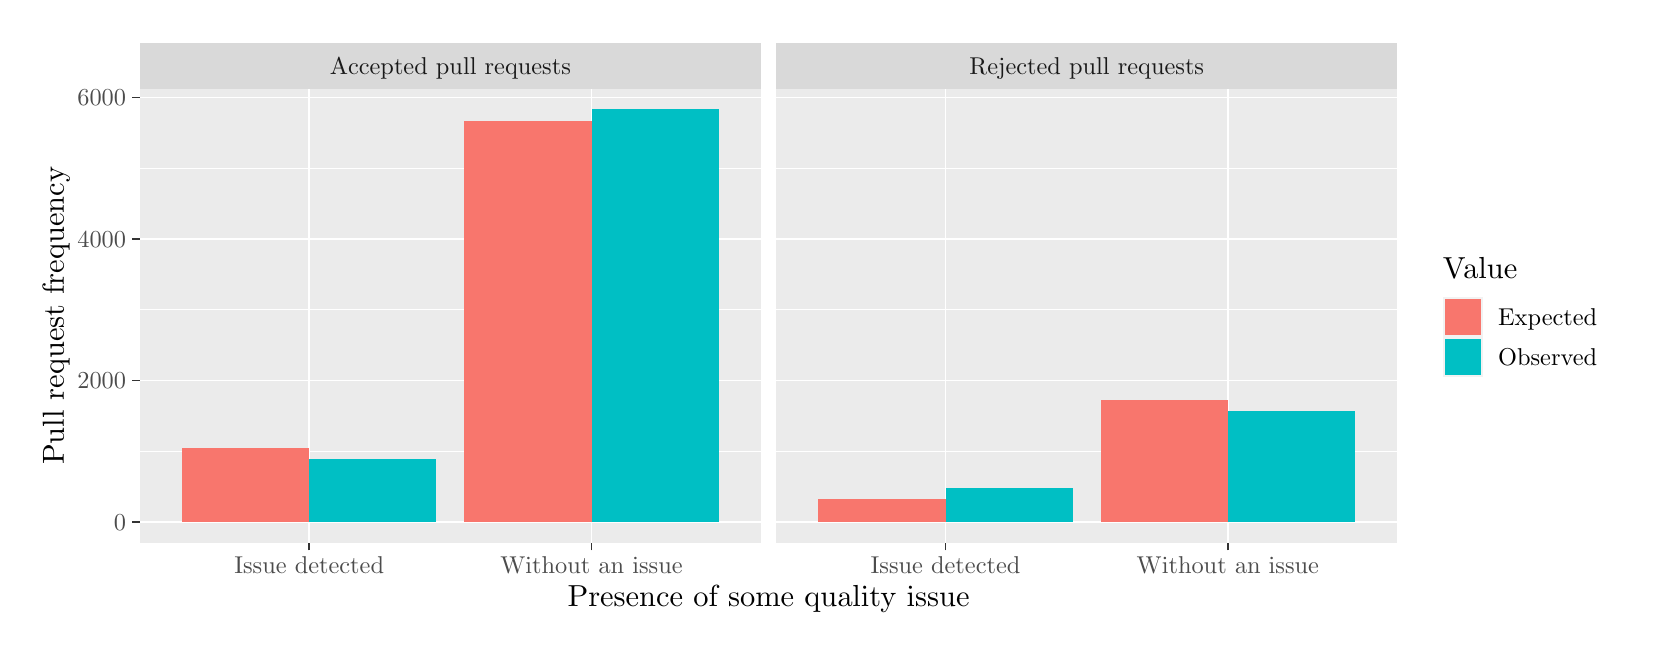
\begin{tikzpicture}[x=1pt,y=1pt]
\definecolor{fillColor}{RGB}{255,255,255}
\path[use as bounding box,fill=fillColor,fill opacity=0.00] (0,0) rectangle (578.16,216.81);
\begin{scope}
\path[clip] (  0.00,  0.00) rectangle (578.16,216.81);
\definecolor{drawColor}{RGB}{255,255,255}
\definecolor{fillColor}{RGB}{255,255,255}

\path[draw=drawColor,line width= 0.6pt,line join=round,line cap=round,fill=fillColor] (  0.00,  0.00) rectangle (578.16,216.81);
\end{scope}
\begin{scope}
\path[clip] ( 40.51, 30.69) rectangle (264.96,194.74);
\definecolor{fillColor}{gray}{0.92}

\path[fill=fillColor] ( 40.51, 30.69) rectangle (264.96,194.74);
\definecolor{drawColor}{RGB}{255,255,255}

\path[draw=drawColor,line width= 0.3pt,line join=round] ( 40.51, 63.71) --
	(264.96, 63.71);

\path[draw=drawColor,line width= 0.3pt,line join=round] ( 40.51,114.85) --
	(264.96,114.85);

\path[draw=drawColor,line width= 0.3pt,line join=round] ( 40.51,165.98) --
	(264.96,165.98);

\path[draw=drawColor,line width= 0.6pt,line join=round] ( 40.51, 38.14) --
	(264.96, 38.14);

\path[draw=drawColor,line width= 0.6pt,line join=round] ( 40.51, 89.28) --
	(264.96, 89.28);

\path[draw=drawColor,line width= 0.6pt,line join=round] ( 40.51,140.42) --
	(264.96,140.42);

\path[draw=drawColor,line width= 0.6pt,line join=round] ( 40.51,191.55) --
	(264.96,191.55);

\path[draw=drawColor,line width= 0.6pt,line join=round] (101.72, 30.69) --
	(101.72,194.74);

\path[draw=drawColor,line width= 0.6pt,line join=round] (203.74, 30.69) --
	(203.74,194.74);
\definecolor{fillColor}{RGB}{0,191,196}

\path[fill=fillColor] (101.72, 38.14) rectangle (147.63, 60.87);

\path[fill=fillColor] (203.74, 38.14) rectangle (249.65,187.28);
\definecolor{fillColor}{RGB}{248,118,109}

\path[fill=fillColor] ( 55.81, 38.14) rectangle (101.72, 64.92);

\path[fill=fillColor] (157.83, 38.14) rectangle (203.74,183.23);
\end{scope}
\begin{scope}
\path[clip] (270.46, 30.69) rectangle (494.90,194.74);
\definecolor{fillColor}{gray}{0.92}

\path[fill=fillColor] (270.46, 30.69) rectangle (494.90,194.74);
\definecolor{drawColor}{RGB}{255,255,255}

\path[draw=drawColor,line width= 0.3pt,line join=round] (270.46, 63.71) --
	(494.90, 63.71);

\path[draw=drawColor,line width= 0.3pt,line join=round] (270.46,114.85) --
	(494.90,114.85);

\path[draw=drawColor,line width= 0.3pt,line join=round] (270.46,165.98) --
	(494.90,165.98);

\path[draw=drawColor,line width= 0.6pt,line join=round] (270.46, 38.14) --
	(494.90, 38.14);

\path[draw=drawColor,line width= 0.6pt,line join=round] (270.46, 89.28) --
	(494.90, 89.28);

\path[draw=drawColor,line width= 0.6pt,line join=round] (270.46,140.42) --
	(494.90,140.42);

\path[draw=drawColor,line width= 0.6pt,line join=round] (270.46,191.55) --
	(494.90,191.55);

\path[draw=drawColor,line width= 0.6pt,line join=round] (331.67, 30.69) --
	(331.67,194.74);

\path[draw=drawColor,line width= 0.6pt,line join=round] (433.69, 30.69) --
	(433.69,194.74);
\definecolor{fillColor}{RGB}{0,191,196}

\path[fill=fillColor] (331.67, 38.14) rectangle (377.58, 50.36);

\path[fill=fillColor] (433.69, 38.14) rectangle (479.60, 78.39);
\definecolor{fillColor}{RGB}{248,118,109}

\path[fill=fillColor] (285.76, 38.14) rectangle (331.67, 46.32);

\path[fill=fillColor] (387.78, 38.14) rectangle (433.69, 82.43);
\end{scope}
\begin{scope}
\path[clip] ( 40.51,194.74) rectangle (264.96,211.31);
\definecolor{fillColor}{gray}{0.85}

\path[fill=fillColor] ( 40.51,194.74) rectangle (264.96,211.31);
\definecolor{drawColor}{gray}{0.10}

\node[text=drawColor,anchor=base,inner sep=0pt, outer sep=0pt, scale=  0.88] at (152.73,199.99) {Accepted pull requests};
\end{scope}
\begin{scope}
\path[clip] (270.46,194.74) rectangle (494.90,211.31);
\definecolor{fillColor}{gray}{0.85}

\path[fill=fillColor] (270.46,194.74) rectangle (494.90,211.31);
\definecolor{drawColor}{gray}{0.10}

\node[text=drawColor,anchor=base,inner sep=0pt, outer sep=0pt, scale=  0.88] at (382.68,199.99) {Rejected pull requests};
\end{scope}
\begin{scope}
\path[clip] (  0.00,  0.00) rectangle (578.16,216.81);
\definecolor{drawColor}{gray}{0.20}

\path[draw=drawColor,line width= 0.6pt,line join=round] (101.72, 27.94) --
	(101.72, 30.69);

\path[draw=drawColor,line width= 0.6pt,line join=round] (203.74, 27.94) --
	(203.74, 30.69);
\end{scope}
\begin{scope}
\path[clip] (  0.00,  0.00) rectangle (578.16,216.81);
\definecolor{drawColor}{gray}{0.30}

\node[text=drawColor,anchor=base,inner sep=0pt, outer sep=0pt, scale=  0.88] at (101.72, 19.68) {Issue detected};

\node[text=drawColor,anchor=base,inner sep=0pt, outer sep=0pt, scale=  0.88] at (203.74, 19.68) {Without an issue};
\end{scope}
\begin{scope}
\path[clip] (  0.00,  0.00) rectangle (578.16,216.81);
\definecolor{drawColor}{gray}{0.20}

\path[draw=drawColor,line width= 0.6pt,line join=round] (331.67, 27.94) --
	(331.67, 30.69);

\path[draw=drawColor,line width= 0.6pt,line join=round] (433.69, 27.94) --
	(433.69, 30.69);
\end{scope}
\begin{scope}
\path[clip] (  0.00,  0.00) rectangle (578.16,216.81);
\definecolor{drawColor}{gray}{0.30}

\node[text=drawColor,anchor=base,inner sep=0pt, outer sep=0pt, scale=  0.88] at (331.67, 19.68) {Issue detected};

\node[text=drawColor,anchor=base,inner sep=0pt, outer sep=0pt, scale=  0.88] at (433.69, 19.68) {Without an issue};
\end{scope}
\begin{scope}
\path[clip] (  0.00,  0.00) rectangle (578.16,216.81);
\definecolor{drawColor}{gray}{0.30}

\node[text=drawColor,anchor=base east,inner sep=0pt, outer sep=0pt, scale=  0.88] at ( 35.56, 35.11) {0};

\node[text=drawColor,anchor=base east,inner sep=0pt, outer sep=0pt, scale=  0.88] at ( 35.56, 86.25) {2000};

\node[text=drawColor,anchor=base east,inner sep=0pt, outer sep=0pt, scale=  0.88] at ( 35.56,137.38) {4000};

\node[text=drawColor,anchor=base east,inner sep=0pt, outer sep=0pt, scale=  0.88] at ( 35.56,188.52) {6000};
\end{scope}
\begin{scope}
\path[clip] (  0.00,  0.00) rectangle (578.16,216.81);
\definecolor{drawColor}{gray}{0.20}

\path[draw=drawColor,line width= 0.6pt,line join=round] ( 37.76, 38.14) --
	( 40.51, 38.14);

\path[draw=drawColor,line width= 0.6pt,line join=round] ( 37.76, 89.28) --
	( 40.51, 89.28);

\path[draw=drawColor,line width= 0.6pt,line join=round] ( 37.76,140.42) --
	( 40.51,140.42);

\path[draw=drawColor,line width= 0.6pt,line join=round] ( 37.76,191.55) --
	( 40.51,191.55);
\end{scope}
\begin{scope}
\path[clip] (  0.00,  0.00) rectangle (578.16,216.81);
\definecolor{drawColor}{RGB}{0,0,0}

\node[text=drawColor,anchor=base,inner sep=0pt, outer sep=0pt, scale=  1.10] at (267.71,  7.64) {Presence of some quality issue};
\end{scope}
\begin{scope}
\path[clip] (  0.00,  0.00) rectangle (578.16,216.81);
\definecolor{drawColor}{RGB}{0,0,0}

\node[text=drawColor,rotate= 90.00,anchor=base,inner sep=0pt, outer sep=0pt, scale=  1.10] at ( 13.08,112.71) {Pull request frequency};
\end{scope}
\begin{scope}
\path[clip] (  0.00,  0.00) rectangle (578.16,216.81);
\definecolor{fillColor}{RGB}{255,255,255}

\path[fill=fillColor] (505.90, 85.15) rectangle (572.66,140.27);
\end{scope}
\begin{scope}
\path[clip] (  0.00,  0.00) rectangle (578.16,216.81);
\definecolor{drawColor}{RGB}{0,0,0}

\node[text=drawColor,anchor=base west,inner sep=0pt, outer sep=0pt, scale=  1.10] at (511.40,126.13) {Value};
\end{scope}
\begin{scope}
\path[clip] (  0.00,  0.00) rectangle (578.16,216.81);
\definecolor{fillColor}{gray}{0.95}

\path[fill=fillColor] (511.40,105.11) rectangle (525.86,119.56);
\end{scope}
\begin{scope}
\path[clip] (  0.00,  0.00) rectangle (578.16,216.81);
\definecolor{fillColor}{RGB}{248,118,109}

\path[fill=fillColor] (512.11,105.82) rectangle (525.15,118.85);
\end{scope}
\begin{scope}
\path[clip] (  0.00,  0.00) rectangle (578.16,216.81);
\definecolor{fillColor}{gray}{0.95}

\path[fill=fillColor] (511.40, 90.65) rectangle (525.86,105.11);
\end{scope}
\begin{scope}
\path[clip] (  0.00,  0.00) rectangle (578.16,216.81);
\definecolor{fillColor}{RGB}{0,191,196}

\path[fill=fillColor] (512.11, 91.36) rectangle (525.15,104.39);
\end{scope}
\begin{scope}
\path[clip] (  0.00,  0.00) rectangle (578.16,216.81);
\definecolor{drawColor}{RGB}{0,0,0}

\node[text=drawColor,anchor=base west,inner sep=0pt, outer sep=0pt, scale=  0.88] at (531.36,109.30) {Expected};
\end{scope}
\begin{scope}
\path[clip] (  0.00,  0.00) rectangle (578.16,216.81);
\definecolor{drawColor}{RGB}{0,0,0}

\node[text=drawColor,anchor=base west,inner sep=0pt, outer sep=0pt, scale=  0.88] at (531.36, 94.85) {Observed};
\end{scope}
\end{tikzpicture}
